% !Mode:: "TeX:UTF-8"
% !TEX root = ../main.tex
\chapter{多孔圆柱绕流的数值求解模型}

\section{问题描述}

\subsection{控制方程} % homogenous fluid region, and porous region

\subsection{边界条件} % Including interface between the homogeneous fluid and porous medium regions

\section{离散方法}

\subsection{时间的离散}

\subsection{空间的离散}

\section{求解模型} %即求解器?SIMPLE

\section{网格划分}

\subsection{网格生成}

流动区域设定为边长 60 的正方形。为了获得圆柱内外的流动状态,流动区域被划分为三块,其中有两块位于圆柱内部,一块位于圆柱外部,见图~\ref{fig: grid}。网格尺寸见表~\ref{tab: grid}。雷诺数和达西数分别为 100 和 0.0001。
\begin{figure}
	\centering
	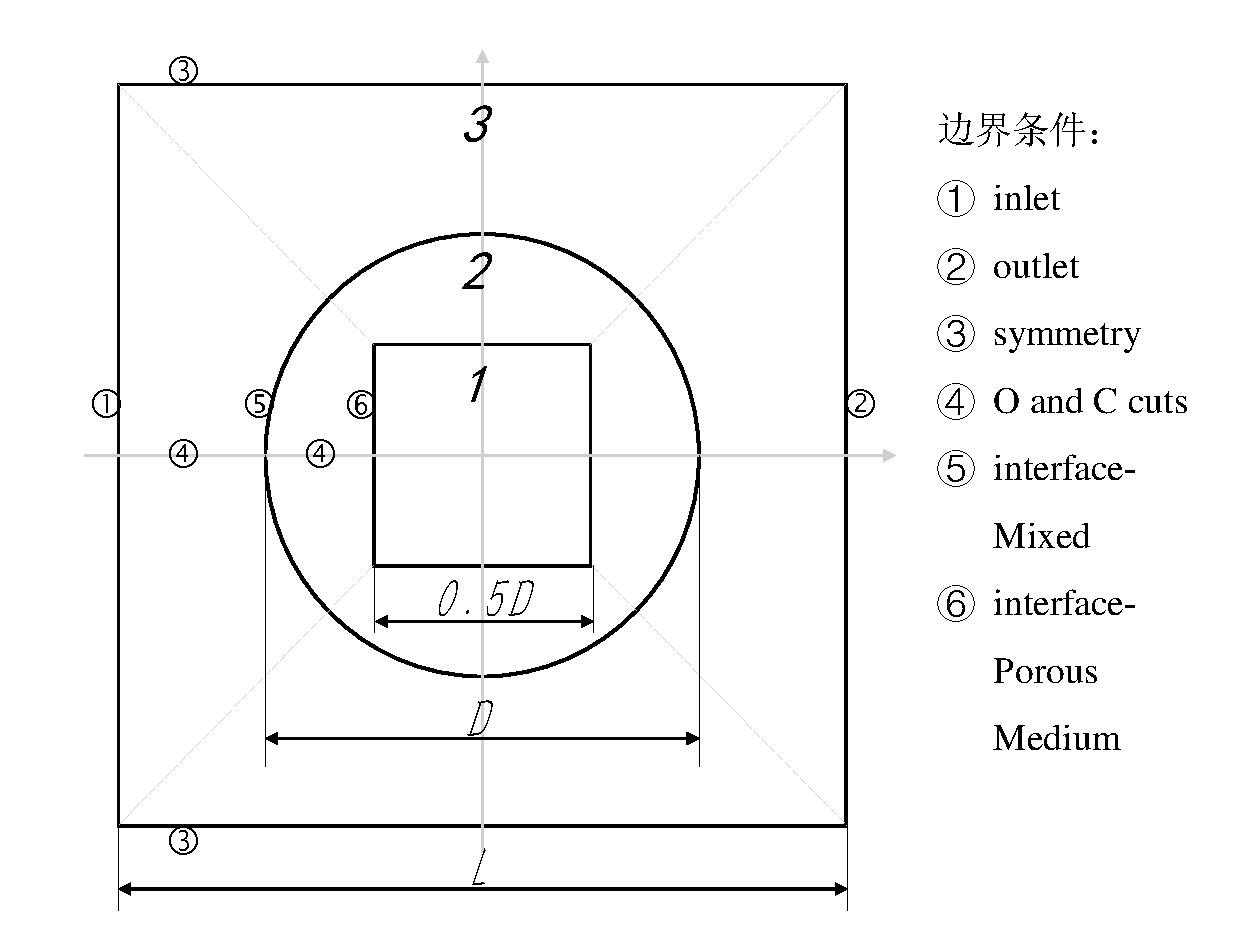
\includegraphics[scale=.6]{../diagrams/grid}
	\caption{网格划分}\label{fig: grid}
\end{figure}

\subsection{网格无关性分析}

\begin{table}
	\caption{网格尺寸}\label{tab: grid}
	\vspace{.5em}\centering\wuhao
	\begin{tabular}{ccccc}
		\toprule[1.5pt]
		\multirow{2}[3]{*}{序号} & \multicolumn{3}{c}{网格尺寸} & \multirow{2}[3]{*}{平均阻力系数} \\
		\cmidrule[.67pt](lr){2-4}
		& Block 1 & Block 2 & Block 3 & \\
		\midrule[1pt]
		1 & 40 $\times$ 40 & 160 $\times$ 25 & 160 $\times$ 140 & 1.2354 \\
		2 & 60 $\times$ 60 & 240 $\times$ 30 & 240 $\times$ 170 & 1.2426 \\
		3 & 80 $\times$ 80 & 320 $\times$ 40 & 320 $\times$ 200 & 1.2462 \\
		4 & 100 $\times$ 100 & 400 $\times$ 50 & 400 $\times$ 230 & 1.2417 \\
		\bottomrule[1.5pt]
	\end{tabular}
\end{table}

\section{结果验证}

\section{本章小结}
